\section{Follow-up Stages: Repairing the Agent and Re-testing the Gate (V2, V3)}
\label{sec:followup}
\paragraph*{Progression and evidence status}
Sections~\ref{sec:hyp}--\ref{sec:explore} report stage~V1, the pre-specified confidence-gate study. Its negative result changed the project's question in two steps. V2 asked whether fixing the weaknesses that V1 exposed makes the agent stronger, and which fix matters. V3 returned to the original question with a better gate and added a control for whether System~1 contributes at all once V2's repairs exist. V1 is retained unchanged as the confirmatory study; V2 and V3 each have their own protocol (\path{docs/V2_PROTOCOL.md}, \path{docs/V3_PROTOCOL.md}) committed before the corresponding test runs, with the same self-registration caveat as in Section~\ref{sec:hyp}.

The three stages are not directly comparable. Each used a different, previously unused test month, a different number of positions, a different opening set and (in V3) a different anchor set (Table~\ref{tab:stages}). ACPL and Elo are therefore compared \emph{within} a stage, never across stages. V1 was reproduced from its raw result files. For V2 and V3 we recomputed the move-quality, gate and rating statistics from the per-position and per-game files of the development laptop (84 numerical checks, none failed; Appendix~\ref{app:evidence}), using the project's own Elo code and the frozen gate weights. Two kinds of quantity were not recomputed: development-stage figures that appear only in the deviations log and protocols, and the learned-gate cross-validation figures.

\begin{table*}[t]
\centering
\caption{The three stages. Test positions and openings are disjoint between stages and from all development data. ``Evidence'' states what we could check; Appendix~\ref{app:evidence} gives details. $^{\natural}$Elo values are on an anchor-relative scale that is not shared across stages.}
\label{tab:stages}
\small
\begin{tabular}{@{}>{\raggedright\arraybackslash}p{0.8cm}>{\raggedright\arraybackslash}p{3.2cm}>{\raggedright\arraybackslash}p{5.2cm}>{\raggedright\arraybackslash}p{3.5cm}>{\raggedright\arraybackslash}p{3.2cm}@{}}
\toprule
 & Question & Agent changes & Test data & Evidence \\
\midrule
V1 & Does System~1 confidence tell when to search? & Confidence gate (Section~\ref{sec:arch}) & 2025-11; 3{,}000 positions; 25 openings; anchor 1320; 500 games & Reproduced from raw files (70 checks) \\
V2 & Can targeted fixes make the agent stronger? & Blunder filter, tablebases, mate-in-one, contempt, quiescence leaves, tactical priors, hand-written criticality gate, retrained value net & 2025-03; 2{,}000 positions; 50 openings; anchor 1320; 600 games & Recomputed from per-position and per-game files \\
V3 & Can a learned gate decide when to search? Does System~1 matter? & Logistic gate over 18 pre-search features; classical-policy control; second anchor & 2025-02; 2{,}000 positions; 50 openings; anchors 1320, 1600; 800 games & Recomputed from per-position and per-game files \\
\bottomrule
\end{tabular}
\end{table*}

\subsection{V2: repairing the diagnosed weaknesses}
\paragraph*{Design}
Each V2 component answers one V1 finding: 17.3\% of System~1 moves were blunders that search barely repaired (blunder filter); leaves were evaluated mid-exchange and interior priors were uniform (quiescence, tactical priors); confidence did not locate search gains, which lay in sharp positions and endgames (criticality gate); the value network was constant on 9.2\% of test positions (retrained); search helped most in endgames (tablebases, mate-in-one); and 74\% of round-robin games ended in repetition (contempt). Only the root-prior temperature was tuned. The decision flow is in Section~\ref{sec:arch-v2}. V2 was developed on V1 validation positions and V1 openings only, then frozen before the fresh-month runs (tag \texttt{v2-frozen}).

\paragraph*{Development decisions and deviations}
The retrained value network met the pre-specified Spearman criterion against Stockfish on validation (0.665 against 0.619 for the V1 network) but missed the dead-head criterion (1.3\% against the required $<1\%$). With a LeakyReLU head an inactive hidden layer no longer forces a constant output, and the constant-output rate was 0.0\% (V1 network on the same check: 8.1\%); the network was accepted and the miss logged. The root-prior temperature was chosen on the first 300 validation positions, ACPL 75.3 at 0.01 against 68.8 at 0.1, so 0.1 was frozen. This choice used the same positions that report it and the figures are optimistic. The first launch of the V2 tournaments exhausted memory before any game was played and was relaunched as two staggered processes; no result was affected.

\paragraph*{Move quality (Study~A-v2)}
On 2{,}000 fresh positions, the blunder filter alone (\ag{v2_safe}, no search) lowers ACPL from 114.5 to 76.5 and the blunder rate from 17.7\% to 11.5\% (Table~\ref{tab:v2a}). Adding the criticality gate and the improved search (\ag{v2_full}) lowers ACPL to 68.7, and searching on every move (\ag{v2_always}) to 65.4. The three differences from System~1 alone have paired 95\% intervals that exclude zero. Paired intervals between V2 agents, recomputed from the per-position data, are $-7.8$\cp\ [$-11.7$, $-4.2$] for \ag{v2_full} against \ag{v2_safe}, $-3.3$ [$-5.5$, $-1.1$] for \ag{v2_always} against \ag{v2_full}, and $+1.0$ [$-1.1$, $+3.1$] for the old network against the retrained one. The 7.8\cp\ gain from search and gating on top of the filter is therefore distinguishable from zero, but it bundles several changes (criticality gate, quiescence, tactical priors, temperature 0.1, new value network) that were not separated experimentally. On top of the filter, search helps in endgames (ACPL 64.5 to 53.8) and middlegames (91.8 to 82.0) and does not help in openings (42.5 to 43.5); by-phase figures are from the project's \path{V2_studyA_by_phase.csv}.

\begin{table}[t]
\centering
\caption{Study~A-v2 (fresh month 2025-03, 2{,}000 positions per agent; read from result files). Bl.\ is the blunder rate, S2 the share of moves searched, ms the mean time per move, and $\Delta$ACPL the paired difference from \ag{laya_only} (bootstrap over positions). $^{\dagger}$Added post hoc after the tournament, on the same positions.}
\label{tab:v2a}
\scriptsize\setlength{\tabcolsep}{2.2pt}\begin{tabular}{lrrrrr}\toprule
Agent & ACPL & Bl.\ \% & $\Delta$ACPL [95\% CI] & S2 \% & ms \\
\midrule
\texttt{laya\_only} & 114.5 & 17.7 & -- & 0 & 476 \\
\texttt{v2\_safe} & 76.5 & 11.5 & -38.1 [-44.9, -31.2] & 0 & 571 \\
\texttt{v2\_full} & 68.7 & 9.6 & -45.9 [-53.6, -38.2] & 60 & 1308 \\
\texttt{v2\_always} & 65.4 & 9.2 & -49.1 [-57.2, -41.2] & 99 & 1604 \\
\texttt{v2\_full\_oldnet}$^{\dagger}$ & 69.7 & 9.7 & -44.8 [-52.4, -37.3] & 60 & 1166 \\
\bottomrule\end{tabular}

\end{table}

\paragraph*{Playing strength (Tournament-v2)}
Against the 1320 anchor, \ag{v2_full} scored 25.0\% against 9.5\% for \ag{laya_only}, and beat \ag{laya_only} head-to-head by 76 points to 24 over 100 games. Table~\ref{tab:stageelo} places it about 200 Elo above \ag{laya_only} (1130 against 930). The \ag{laya_only} rating is flagged off-scale because it scored under 10\% against the only anchor, so the size of the gap is an extrapolation although its direction is not in doubt. Games ended by threefold repetition in 142 of 600 cases against 74.3\% of V1 round-robin games, but V1's figure came from games between our own deterministic agents, so the two are not comparable. Whether contempt caused the drop was not tested (its ablation was not run).

Two ablations bear on what matters. The V1 value network inside the V2 agent (\ag{v2_full_oldnet}) is statistically indistinguishable from the retrained one: 1.0\cp\ worse in Study~A and 39 Elo higher in games, both well inside the intervals. The agent's strength no longer depends visibly on the value network. Removing the blunder filter from \ag{v2_full} (\ag{v2_full_nosafety}) leaves 1080 Elo, roughly equal to the filter without search (\ag{v2_safe}, 1069), with 100 games each and intervals of about $\pm70$ Elo. The project's summary that the blunder filter ``gives most of the gain'' is supported for move quality (Study~A) but not isolated for playing strength: \ag{v2_safe} also contains tablebases, mate-in-one and contempt, and \ag{v2_full_nosafety} retains them, so neither pair of agents separates the filter from those rules.

\paragraph*{Scrutiny of the V2 gate (post hoc)}
V1's negative result raised the question of whether the criticality gate also fails the matched-random control, which V2 had not included. A post hoc script reported that the criticality gate at its 60\% search rate is not distinguishable from a random gate at the same rate ($+1.1$\cp, 95\% CI $[-2.4,+4.7]$), while a hindsight oracle at that rate would reach ACPL 52.6 against 68.7. We reproduced these figures from the per-position data (point estimate $+1.10$, oracle 52.6, interval $[-2.3,+4.8]$ with the same fresh-random-gate procedure). With the lower-variance analytic comparison used below the interval is $[-0.8,+3.1]$, which still contains zero.

\subsection{V3: a learned gate, a classical control and a second anchor}
\paragraph*{Design}
The V3 gate is a logistic model $g(\mathbf{x})=\sigma(\mathbf{w}^{\top}\mathbf{x}+b)$ that predicts whether searching improves the move, i.e.\ whether $\mathrm{CPL}_{\text{safe}}-\mathrm{CPL}_{\text{always}}>0$. It takes 18 features available before search (System~1 win-chance margins, entropy and confidence, legal-move and capture counts, the five criticality flags, material, ply, whether the filter overrides System~1, two tactical-score summaries) and was trained on the 3{,}000 V1 validation positions with five-fold cross-validation grouped by game; a ridge model was the alternative. Thresholds for 10\%, 25\% and 60\% search rates were set on validation. The largest weights favour search when System~1 cannot separate its top moves (margin $-1.76$, confidence $-1.28$), the same direction as V1's confidence gate. Composed validation ACPL under cross-validation was 74.2/71.7/68.3 for the learned gate against 76.5/74.6/70.2 for a random gate at 10/25/60\%.

Two V3 engine options were tested on validation positions against rules fixed in advance (adopt only if $\ge2$\cp\ better and $\le30\%$ slower) and rejected: extending the filter's search with checks (0.3\cp), and a System~1 two-ply look-ahead (1.4--4.8\cp\ for 27--59\% more time). The look-ahead was run on the test set as the labelled exploratory agent \ag{v3_look4}, ACPL 64.5 (Study~A only).

The tournament added \ag{classical_full}, the same filter and search driven by a hand-written heuristic policy instead of System~1, to test whether System~1 matters once the filter exists, and a second anchor at Elo 1600.

\paragraph*{An invalid first run, reported}
The first V3 test run was invalid. The generated configuration had silently reset the root-prior temperature to 0.01, V1's value, overwriting the V2 choice (0.1), because a later code handoff replaced the generator script. Search then agreed with the filter's move on 92.8\% of positions and gained 1.55\cp\ on average instead of 11.7\cp\ in the valid re-run (both recomputed from the saved files; the re-run agrees on 55\% of positions). The run (kept as \texttt{v3\_bench\_T001\_INVALID}) yielded a learned-gate advantage of only $+0.5$ to $+0.7$\cp\ over random, and did not test the frozen design. The setting was restored and Study~A and the tournaments were re-run on the same 2025-02 sets with the same frozen gate. The invalid result had been seen before the re-run, and we report both. The failure is informative: a root-prior temperature of 0.01 makes search nearly inert, which supports the reading of V1's small search effect (8.2\% of moves changed) offered in Section~\ref{sec:arch}, although V1 never tested that link directly.

\paragraph*{Gate results (Q1)}
The pre-specified primary question was whether the learned gate beats a random gate at the same rate, tested at 25\% with Holm correction over 10/25/60\%. Under the pre-registered procedure it does not (Table~\ref{tab:v3gate}, left block): the advantage is $+2.5$\cp\ [$-0.9$, $+5.8$], $p=0.069$, and after Holm adjustment no rate is significant. We reproduced these figures exactly from the per-position data and the frozen gate weights. That procedure draws a fresh random gate inside every bootstrap resample, so its interval includes the sampling noise of one random mask. This is the same noise that the V1 analysis removed by using the expectation over random gates (Section~\ref{sec:methods}).

Applying that expectation-based (analytic) test to the same V3 data, a post hoc analysis that was not pre-specified, gives narrower intervals (Table~\ref{tab:v3gate}, right block): $+2.5$\cp\ [$+0.4$, $+4.7$] at 25\% (Holm $p=0.021$) and $+3.2$\cp\ [$+1.4$, $+4.9$] at 60\% (Holm $p<0.001$), with the 10\% rate not significant ($p=0.063$). Resampling the 1{,}696 games instead of positions leaves this unchanged (25\%: $[+0.4,+4.6]$). The point estimates are identical in the two analyses; only the width of the interval differs. We therefore report both: the pre-registered verdict, that the primary comparison is not supported, stands, and the post hoc analysis indicates a real but modest advantage over random gating of about 2.5\cp\ at a 25\% rate. The learned gate closes about 12\% of the gap between a random gate and the hindsight oracle at 25\% ($2.5/20.2$\cp). The same analytic test also puts the hand-written criticality gate ahead of random on the V3 positions ($+2.5$\cp\ [$+0.6$, $+4.5$] at its 57.6\% rate) but not on the V2 positions ($+1.1$ [$-0.8$, $+3.1$] at 60\%), so the evidence for a learned gate over a hand-written one is not established, and we did not test them against each other.

\begin{table*}[t]
\centering
\caption{V3 test, composed ACPL on 2{,}000 positions of 2025-02, recomputed from the per-position files. Advantage is random minus learned (cp; $>0$ favours the learned gate); $p$ is one-sided; Holm over the three rates. Pre-registered test: a fresh random gate per resample (reproduces the project's logged output). Analytic test (post hoc): expectation over random gates, 4{,}000 position resamples. Reference ACPL: never search 76.6, critical gate (57.6\%) 67.4, always search 64.9. $^{*}$Primary comparison. $^{\S}$Hindsight oracle, not achievable.}
\label{tab:v3gate}
\scriptsize\setlength{\tabcolsep}{2.2pt}\begin{tabular}{rrrrrrrrrr}\toprule
 & & & & \multicolumn{3}{c}{Pre-registered test} & \multicolumn{3}{c}{Analytic test (post hoc)} \\
\cmidrule(lr){5-7}\cmidrule(lr){8-10}
Rate (\%) & Learned & Random & Oracle$^{\S}$ & Advantage [95\% CI] & $p$ & Holm & Advantage [95\% CI] & $p$ & Holm \\
\midrule
10 & 74.1 & 75.4 & 57.1 & +1.3 [-1.2, +3.9] & 0.149 & 0.149 & +1.3 [-0.3, +3.1] & 0.063 & 0.063 \\
25$^{*}$ & 71.1 & 73.6 & 53.4 & +2.5 [-0.9, +5.8] & 0.069 & 0.138 & +2.5 [+0.4, +4.7] & 0.010 & 0.021 \\
60 & 66.4 & 69.6 & 53.4 & +3.2 [+0.1, +6.7] & 0.022 & 0.066 & +3.2 [+1.4, +4.9] & $<$0.001 & $<$0.001 \\
\bottomrule\end{tabular}

\end{table*}

\paragraph*{Strength and the role of System~1 (Q2--Q4)}
Table~\ref{tab:stageelo} and Table~\ref{tab:v3diff} give the V3 ratings and the paired differences (a shared bootstrap over openings, computed by a script written after the run because per-agent intervals cannot be subtracted). In games the learned gate searched on 39.8\% of moves, not the 25\% it was calibrated for, because positions arising in play look uncertain to it more often than benchmark positions; the same effect appeared for the V1 gate (Section~\ref{sec:studyb}). It matched \ag{v2_full} in rating ($-3$ Elo) at about 20\% less time per move (0.91 against 1.13 s), but the interval ($-89$ to $+81$) is far too wide to show equivalence, so Q2 is inconclusive. Replacing System~1 by the hand-written policy costs about 212 Elo [133, 296] (Q3), so System~1 does contribute, and the filter overrode the heuristic policy on 35.7\% of its moves against 9\% for System~1-driven \ag{v2_full}. The V2 comparison replicates on a second month and under two anchors: \ag{v2_full} is 289 Elo [208, 380] above \ag{laya_only} (Q4), with Study~A ACPL $111.8\to67.4$ and blunders $17.4\%\to9.7\%$, close to V2's $114.5\to68.7$ and $17.7\%\to9.6\%$. Study~A did not run the live \ag{v3_learned_25} and \ag{classical_full} agents; the learned gate's ACPL is the offline composition from the other agents' moves.

\begin{table}[t]
\centering
\caption{Ratings by stage. Elo is anchor-relative and each panel has its own opponents and openings; compare differences within a panel only. $^{\ddagger}$Scored under 10\% against the anchor (off-scale). Each V3 agent played 100 games against each of two anchors; the last two columns give its score against each.}
\label{tab:stageelo}
\scriptsize\setlength{\tabcolsep}{2.2pt}\begin{tabular}{lrrrr}\toprule
Agent & Elo [95\% CI] & Games & vs.\ 1320 (\%) & vs.\ 1600 (\%) \\
\midrule
\multicolumn{5}{l}{\textit{V2, test month 2025-03; anchor 1320 only}}\\
\texttt{laya\_only}$^{\ddagger}$ & 930 [863, 984] & 200 & 9.5 & -- \\
\texttt{v2\_safe} & 1069 [1005, 1125] & 100 & 19.0 & -- \\
\texttt{v2\_full\_nosafety} & 1080 [998, 1148] & 100 & 20.0 & -- \\
\texttt{v2\_full} & 1130 [1072, 1180] & 200 & 25.0 & -- \\
\texttt{v2\_full\_oldnet} & 1169 [1090, 1235] & 100 & 29.5 & -- \\
\midrule\multicolumn{5}{l}{\textit{V3, test month 2025-02; anchors 1320 and 1600}}\\
\texttt{laya\_only}$^{\ddagger}$ & 903 [825, 966] & 200 & 7 & 3 \\
\texttt{classical\_full} & 980 [912, 1036] & 200 & 11 & 4 \\
\texttt{v2\_full} & 1192 [1145, 1236] & 200 & 26 & 15 \\
\texttt{v3\_learned\_25} & 1189 [1128, 1251] & 200 & 24.5 & 16 \\
\bottomrule\end{tabular}

\end{table}

\begin{table}[t]
\centering
\caption{V3 paired Elo differences. Q2: inconclusive, since the interval includes $-50$.}
\label{tab:v3diff}
\scriptsize\setlength{\tabcolsep}{2.2pt}\begin{tabular}{lrl}\toprule
Contrast & $\Delta$Elo [95\% CI] & Status \\
\midrule
v3\_learned\_25 $-$ v2\_full & -3 [-89, +81] & Q2 \\
v2\_full $-$ classical\_full & +212 [+133, +296] & Q3 \\
v2\_full $-$ laya\_only & +289 [+208, +380] & Q4 \\
classical\_full $-$ laya\_only & +76 [-33, +190] & exploratory \\
\bottomrule\end{tabular}

\end{table}

\begin{figure*}[t]
\centering
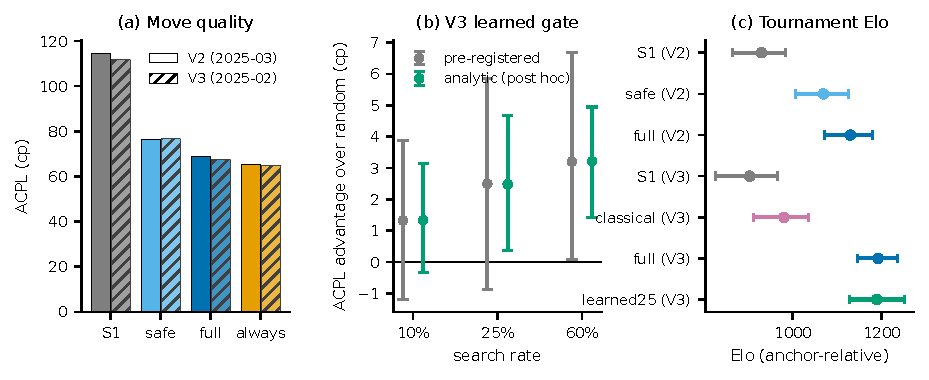
\includegraphics[width=\textwidth]{fig_stages}
\caption{Stages V2 and V3 (different test months and opponents; compare within an agent family, not across stages). (a) ACPL. S1 is \ag{laya_only}, safe is the blunder filter without search, full adds the gate and search, always searches on every move. (b) V3 learned-gate ACPL advantage over a random gate with 95\% intervals under the pre-registered and the analytic (post hoc) procedures; the point estimates are the same. (c) Tournament Elo with 95\% cluster-bootstrap intervals against Stockfish anchors; S1 is off-scale in both stages.}
\label{fig:stages}
\end{figure*}

\subsection{Three gates, one partial answer}
Across the three stages the gating question received a mostly negative and, in the last stage, a modest positive answer. The V1 confidence gate was $-0.09$\cp\ [$-1.30$, $+1.11$] from random at a 52\% rate, under the expectation-based comparison. The V2 criticality gate was $+1.1$\cp\ [$-0.8$, $+3.1$] at 60\% (post hoc). The V3 learned gate was $+2.5$\cp\ at 25\%: not significant under the pre-registered test ($p=0.069$) and significant under the post hoc analytic test ($[+0.4,+4.7]$). These comparisons use different systems, test sets and rates, and only V1 and the V3 primary comparison were pre-specified, so they are not a sequence of improvements. The learned gate has the clearest evidence of an advantage over random gating among the gates studied, but it recovers only about an eighth of the oracle headroom, and what produced a large gain was not a gate but a shallow material check in front of System~1.
